\chapter{VBO}
\begin{tabular}{lcccc}
			& Kartesische Koord. 	& Farben 		& Textur-Koord. & Normal			\\
	$v_0$	& $x_0, y_0,z_0,w_0 $	& $r_0,g_0,b_0$	& $s_0,t_0$		& $u_0, v_0, w'_0$	\\
	$v_1$	&						&				&				&					\\
	$\vdots$&						&				&				&					\\
	$v_{n-1}$&						&				&				&					
\end{tabular}

\begin{tikzpicture}
\end{tikzpicture}

\begin{figure}[H]
	\centering
	\begin{tikzpicture}
\begin{axis}[clip = false, axis lines = none, xmin = 0, xmax = 2, ymin=0, ymax=2]
%\addplot {};
\draw (axis cs:0,0) -- (axis cs:1,2) -- (axis cs:2,0.5) -- (axis cs:0,0);
\draw[xstep = 10, ystep = 10, gray, very thin] (axis cs:0,0) grid (axis cs:2,2);
\node[anchor=north] at (axis cs:0,0) {$V_0$};
\node at (axis cs:0.5,0.5) {x};
\node[anchor=west] at (axis cs:2,0.5) {$V_1$};
\node[anchor=south] at (axis cs:1,2) {$V_2$};
\node[anchor=north] at (axis cs:0,-0.2) {r};
\node[anchor=west] at (axis cs:2.1,0.4) {g};
\node[anchor=south] at (axis cs:1.1,2.2) {b};
\end{axis}
\end{tikzpicture}
\caption{Beispiel Raster?}
\end{figure}

\section{Baryzentrische Koordinaten}
\begin{figure}[H]
	\centering
	\begin{tikzpicture}
\begin{axis}[clip = false, axis lines = none, xmin = 0, xmax = 2, ymin=0, ymax=2]
%\addplot {};
\draw (axis cs:0,0) -- (axis cs:1,2) -- (axis cs:2,0.5) -- (axis cs:0,0);
\node[anchor=north] at (axis cs:0,0) {a};
\node[anchor=west] at (axis cs:2,0.5) {b};
\node[anchor=south] at (axis cs:1,2) {c};
\node at (axis cs:0.5,0.5) {x};
\node[anchor=north] at (axis cs:0,-0.2) {f(a)};
\node[anchor=west] at (axis cs:2.1,0.4) {f(b)};
\node[anchor=south] at (axis cs:1.1,2.2) {f(c)};
\end{axis}
\end{tikzpicture}
\caption{Baryzentrisches Koordinatensystem}
\end{figure}
\[ \vektor{a_1&b_1&c_1\\a_2&b_2&c_2\\1&1&1} \cdot \dddvec{\alpha}{\beta}{\gamma} = \dddvec{x_1}{x_2}{1} \]
\[ x = \alpha\cdot a + \beta \cdot b + \gamma\cdot c \land  \alpha+\beta+\gamma = 1 \]
\[ \Rightarrow f(x) = \alpha\cdot f(a) + \beta\cdot f(b) + \gamma \cdot f(c) \]
\section{Texturen}
\subsection{Mipmap}
\begin{tikzpicture}[scale=1]
\node[anchor=south] at (4,8) {$w$};
\node[anchor=west] at (8,4) {$h$};
\draw (0,0) rectangle (8,8);
\end{tikzpicture}
\begin{tikzpicture}[scale=1/2]
\node[anchor=south] at (4,8) {$\frac{w}{2}$};
\node[anchor=west] at (8,4) {$\frac{h}{2}$};
\draw (0,0) rectangle (8,8);
\end{tikzpicture}
\begin{tikzpicture}[scale=1/4]
\node[anchor=south] at (4,8) {$\frac{w}{4}$};
\node[anchor=west] at (8,4) {$\frac{h}{4}$};
\draw (0,0) rectangle (8,8);
\end{tikzpicture}
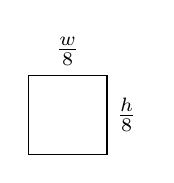
\begin{tikzpicture}[scale=1/8]
\node[anchor=south] at (4,8) {$\frac{w}{8}$};
\node[anchor=west] at (8,4) {$\frac{h}{8}$};
\draw (0,0) rectangle (8,8);
\end{tikzpicture}

\[ S = \sum_{i=0}^{\infty} (\frac{1}{4})^i = \frac{1}{1 - \frac{1}{4}} = \frac{4}{3} \]

\begin{tikzpicture}
\begin{axis}[clip = false, axis lines = none, ylabel={Bildschirmpixel}, xmin = 0, xmax=2, ymin = 0, ymax = 2]
\draw[xstep = 10, ystep = 10, gray, thin] (axis cs:0,0) grid (axis cs:2,2);
\draw[xstep = 50, ystep = 50, gray, very thick] (axis cs:0.5,0.5) grid (axis cs:2,2);
\node[anchor=east] at (axis cs:0,2) {Bildschirmpixel};
\node at (axis cs:0.75,0.75) {\pgfuseplotmark{*}};
\node at (axis cs:1.25,0.75) {\pgfuseplotmark{*}};
\node at (axis cs:1.75,0.75) {\pgfuseplotmark{*}};
\node at (axis cs:0.75,1.25) {\pgfuseplotmark{*}};
\node at (axis cs:1.25,1.25) {\pgfuseplotmark{*}};
\node at (axis cs:1.75,1.25) {\pgfuseplotmark{*}};
\node at (axis cs:0.75,1.75) {\pgfuseplotmark{*}};
\node at (axis cs:1.25,1.75) {\pgfuseplotmark{*}};
\node at (axis cs:1.75,1.75) {\pgfuseplotmark{*}};
\end{axis}
\end{tikzpicture}

\begin{tikzpicture}[scale = 3]
\draw (0,0) rectangle (1,1);
\node[anchor=south east] at (0,1) {$(-1,1)$};
\node[anchor=south west] at (1,1) {$(1,1)$};
\node[anchor=north east] at (0,0) {$(x,y) = (-1,-1)$};
\node[anchor=north west] at (1,0) {$v_0~(1,-1)$};

\node[anchor=south east] at (0,1-0.175) {$(0,0)$};
\node[anchor=south west] at (1,1-0.175) {$(3,0)$};
\node[anchor=north east] at (0,0-0.175) {$(s_3, t_3) = (0,3)$};
\node[anchor=north west] at (1,0-0.175) {$(s_0,t_0) = (3,3) $};
\end{tikzpicture}